%% This is file `elsarticle-template-1-num.tex',
%%
%% Copyright 2009 Elsevier Ltd
%%
%% This file is part of the 'Elsarticle Bundle'.
%% ---------------------------------------------
%%
%% It may be distributed under the conditions of the LaTeX Project Public
%% License, either version 1.2 of this license or (at your option) any
%% later version.  The latest version of this license is in
%%    http://www.latex-project.org/lppl.txt
%% and version 1.2 or later is part of all distributions of LaTeX
%% version 1999/12/01 or later.
%%
%% The list of all files belonging to the 'Elsarticle Bundle' is
%% given in the file `manifest.txt'.
%%
%% Template article for Elsevier's document class `elsarticle'
%% with numbered style bibliographic references
%%
%% $Id: elsarticle-template-1-num.tex 149 2009-10-08 05:01:15Z rishi $
%% $URL: http://lenova.river-valley.com/svn/elsbst/trunk/elsarticle-template-1-num.tex $
%%

%\documentclass[preprint,authoryear,review,12pt]{elsarticle}
 \documentclass[final,5p,times,twocolumn]{elsarticle}

%% Use the option review to obtain double line spacing
%% \documentclass[preprint,review,12pt]{elsarticle}

%% Use the options 1p,two column; 3p; 3p,twocolumn; 5p; or 5p,twocolumn
%% for a journal layout:
%% \documentclass[final,1p,times]{elsarticle}
%% \documentclass[final,1p,times,twocolumn]{elsarticle}
%% \documentclass[final,3p,times]{elsarticle}
%% \documentclass[final,3p,times,twocolumn]{elsarticle}
%% \documentclass[final,5p,times]{elsarticle}
%% \documentclass[final,5p,times,twocolumn]{elsarticle}


\usepackage{color}
\usepackage{multirow,booktabs,ctable,array}
\usepackage{lscape}
\usepackage{amsmath}
\usepackage{lineno}
\usepackage{ulem}
\usepackage{setspace}
\usepackage{listings}
\usepackage{float}
\usepackage{listings}
\usepackage{color}
\usepackage{rccol}
\usepackage[table]{xcolor}
\usepackage{setspace}

    \definecolor{listcomment}{rgb}{0.0,0.5,0.0}
    \definecolor{listkeyword}{rgb}{0.0,0.0,0.5}
    \definecolor{listnumbers}{gray}{0.65}
    \definecolor{listlightgray}{gray}{0.955}
    \definecolor{listwhite}{gray}{1.0}
    
    
\definecolor{Gray}{gray}{0.9}
    

\newcommand{\lstsetcpplong}
{
\lstset{frame = tb,
        framerule = 0.25pt,
        float,
        fontadjust,
        backgroundcolor={\color{listlightgray}},
        basicstyle = {\ttfamily\scriptsize},
        keywordstyle = {\ttfamily\color{listkeyword}\textbf},
        identifierstyle = {\ttfamily},
        commentstyle = {\ttfamily\color{listcomment}\textit},
        stringstyle = {\ttfamily},
        showstringspaces = false,
        showtabs = false,
        numbers = none,
        numbersep = 6pt,
        numberstyle={\ttfamily\color{listnumbers}},
        tabsize = 2,
        language=,
        floatplacement=!h,
        caption={\small \baselineskip 12pt DiReCT long command line menu which is invoked using the `{\ttfamily {-}{-}help}' option.  The short command line menu is obtained by typing `{\ttfamily {-}h}'},
        captionpos=b,
        label=listing:long
        }
}

\floatstyle{plain}
\newfloat{command}{thp}{lop}
\floatname{command}{Command}

%\usepackage[nomarkers,notablist]{endfloat}

%% if you use PostScript figures in your article
%% use the graphics package for simple commands
%% \usepackage{graphics}
%% or use the graphicx package for more complicated commands
%% \usepackage{graphicx}
%% or use the epsfig package if you prefer to use the old commands
%% \usepackage{epsfig}

%% The amssymb package provides various useful mathematical symbols
\usepackage{amssymb}
%% The amsthm package provides extended theorem environments
% \usepackage{amsthm}
 
 \usepackage{makecell}

%% The lineno packages adds line numbers. Start line numbering with
%% \begin{linenumbers}, end it with \end{linenumbers}. Or switch it on
%% for the whole article with \linenumbers after \end{frontmatter}.
%% \usepackage{lineno}

%% natbib.sty is loaded by default. However, natbib options can be
%% provided with \biboptions{...} command. Following options are
%% valid:

%%   round  -  round parentheses are used (default)
%%   square -  square brackets are used   [option]
%%   curly  -  curly braces are used      {option}
%%   angle  -  angle brackets are used    <option>
%%   semicolon  -  multiple citations separated by semi-colon
%%   colon  - same as semicolon, an earlier confusion
%%   comma  -  separated by comma
%%   numbers-  selects numerical citations
%%   super  -  numerical citations as superscripts
%%   sort   -  sorts multiple citations according to order in ref. list
%%   sort&compress   -  like sort, but also compresses numerical citations
%%   compress - compresses without sorting
%%
%% \biboptions{comma,round}

% \biboptions{}

\providecommand{\OO}[1]{\operatorname{O}\bigl(#1\bigr)}

\graphicspath{
             {./Figures/}
             {../SPIE2013/KK/IXI_results/} 
             }

\long\def\symbolfootnote[#1]#2{\begingroup%
\def\thefootnote{\fnsymbol{footnote}}\footnote[#1]{#2}\endgroup}



\journal{NeuroImage}

\begin{document}


\begin{frontmatter}

% \title{The Kapowski Chronicles:  A Complete, Volumetric Cortical Thickness Open Source Pipeline with Evaluation on Public Data}
\title{Large-scale cortical thickness quantification with
  Advanced Normalization Tools (ANTs)}


\author[label1]{Nicholas J.~Tustison
  \fnref{label0}}
  \fntext[label0]{\scriptsize Corresponding author:  PO Box 801339, Charlottesville, VA 22908; T:  434-924-7730; email address:  ntustison@virginia.edu.\\ \\
Partial support provided by US Army Medical Research and Materiel Command; Contract grant number: W81XWH-09-2-0055.
 }
\author[label2]{Philip A.~Cook}
\author[label2]{Gang Song}
\author[label2]{Sandhitsu R.~Das}
\author[label2]{Jeffrey R.~Duda}
\author[label2]{Benjamin M. Kandel}
\author[label3]{Niels van Strien}
\author[label1]{James R.~Stone}
\author[label2]{James C.~Gee}
\author[label2]{Brian B.~Avants}
\address[label1]{Department of Radiology and Medical Imaging, University of Virginia, Charlottesville, VA}
\address[label2]{Penn Image Computing and Science Laboratory, University of Pennsylvania,
                Philadelphia, PA}
\address[label3]{Department of Circulation and Medical Imaging,
  Norwegian University of Science and Technology, Trondheim,
  Norway}




%\maketitle

%\linenumbers


\begin{abstract} 
Numerous studies have explored the relationship between cortical
structure, brain development, cognitive function, and functional
connectivity.  The highly convoluted cortical topography makes manual
measurements arduous and often impractical given the population sizes
necessary for inferring statistical trends.  Computational techniques
have permitted large-scale studies as they provide reproducible
localized measurements characterizing the cortex with little or no
human intervention.  Particularly useful to the neuroscience community
are publicly available tools, such as the popular surface-based
Freesurfer, which facilitate the testing and refinement of hypotheses.
In this paper, we introduce the volume-based Advanced Normalization
Tools (ANTs) cortical thickness automated pipeline comprising
well-vetted components such as SyGN (multivariate template
construction), SyN (image registration), N4 (bias correction), Atropos
($n$-tissue segmentation), and DiReCT (cortical thickness) all
developed as part of the ANTs open science effort.  
We employ cortical thickness as both an outcome measurement and as a reference for validation.  Errors in any previous part of the pipeline will influence the biological plausibility of the final cortical thickness results including the statistical sensitivity of these measurements to demographic variables such as age and gender.  Furthermore, we demonstrate, for the first time, that volumetric cortical thickness measurements are viable and sensitive in large-scale population that span age, gender and image acquisition platforms.
We use
four open data sets (IXI, Kirby, NKI, and Oasis), consisting of approximately 1200
images, in order to evaluate the ANTs cortical thickness pipeline.  
Because ground truth is unavailable in these large datasets, 
we use surrogate measurements to establish validity.  We show that the
pipeline has a low failure rate, has high cortical thickness precision, and produces
reasonable ``BrainAge'' measurements.  DiReCT is also shown to
reveal expected relationships between cortical thickness,
age and gender, in addition to novel gender
differences in predicting structural connectivity across the lifespan.
To further promote open science and use of the proposed tools, all
results and scripts used to produce the results are publicly
available using open science venues.  We also introduce quality assurance/control 
mechanisms, such as the {\it brain constellation map}, for quick assessment
of performance on individual subjects.  Out of over 1200 subjects, we found no severe registration, segmentation or
cortical thickness failures using the proposed methodology.  
\end{abstract}

\begin{keyword}
advanced normalization tools \sep cortical thickness \sep open science
%% keywords here, in the form: keyword \sep keyword
\end{keyword}

\end{frontmatter}
%
%
\newpage


%% MSC codes here, in the form: \MSC code \sep code
%% or \MSC[2008] code \sep code (2000 is the default)

%%
%% Start line numbering here if you want
%%
% \linenumbers

%% The Appendices part is started with the command \appendix;
%% appendix sections are then done as normal sections
%% \appendix

%% \section{}
%% \label{}

%% References
%%
%% Following citation commands can be used in the body text:
%% Usage of \cite is as follows:
%%   \citep{key}          ==>>  [#]
%%   \cite[chap. 2]{key} ==>>  [#, chap. 2]
%%   \citet{key}         ==>>  Author [#]

%% main text

\section{Introduction}

% Neuroscientific investigations into cortical morphological
% changes/differences have illuminated interesting correlations with
% normal and pathological neurodevelopment in  addition to cognitive function.
Historically rooted in the meticulous work of von Economo \citep{economo2008},
imaging-based structural analysis of the brain plays a fundamental role
in identifying the relationship between cortical morphology, disease and cognition.
Discriminative quantitative cortical measures have been demonstrated in conditional 
abnormalities such as 
Huntington's disease \citep{rosas2002,rosas2005,selemon2004}, 
schizophrenia \citep{nesvag2008}, bipolar disorder \cite{lyoo2006}, Alzheimer's disease and frontotemporal
dementia \citep{du2007,dickerson2009}, Parkinson's disease \citep{jubault2011}, Williams syndrome \citep{thompson2005},
multiple sclerosis \citep{ramasamy2009}, autism \citep{chung2005,hardan2006},
migraines \citep{dasilva2007}, chronic smoking \citep{kuhn2010}, alcoholism \citep{fortier2011},
cocaine addiction \citep{makris2008}, Tourette syndrome in children \citep{sowell2008},
scoliosis in
female adolescents \citep{wang2012}, obsessive compulsive
disorder \citep{shin2007}, ADHD \citep{almeida-montes2012}, obesity \citep{raji2010}, and heritable \citep{peterson2009}
and elderly \citep{ballmaier2004} depression.  Cortical thickness also
varies normally as a function of age \citep{kochunov2011},
gender \citep{luders2006a}, untreated
male-to-female transsexuality \citep{luders2012},  handedness
\citep{luders2006,amunts2007}, intelligence \citep{shaw2006}, athletic
ability \citep{wei2011}, musical ability \citep{bermudez2009,foster2010}, 
tendency toward criminality \citep{raine2011}, and Tetris-playing
ability in female adolescents \citep{haier2009}.  Additionally,
recent studies demonstrate structural 
connectivity relationships using cortical thickness measures
\citep{worsley2005,lerch2006,he2007,chen2008}.
Although these findings
are subject to debate and interpretation \citep{gernsbacher2007}, 
the availability of quantitative
computational methods for extracting such information
has proven invaluable for developing and refining fundamental 
neuroscience hypotheses.

Computational methods for analyzing the cortex may be 
broadly characterized as surface mesh-based or volumetric \citep{scott2009,clarkson2011}.  Representative of the former is the
Freesurfer%
\footnote{
http://surfer.nmr.mgh.harvard.edu/
}
cortical modeling software package \citep{dale1999,fischl1999,fischl2000,fischl2002,fischl2004}
which owes its popularity to public availability, excellent documentation, 
good performance, and  integration with other toolkits, such as the extensive FMRIB software 
library (FSL) \citep{smith2004}.  Similar to other surface
approaches (e.g. \cite{davatzikos1996,magnotta1999,macdonald2000,kim2005}), the pial
and white matter surfaces from individual subject MR data are modeled with polygonal meshes  
which are then used to determine local cortical thickness values based on a specified correspondence between 
the surface models.

Image volumetric (or meshless) techniques vary both in algorithmic terms as well as
the underlying definition of cortical thickness.  An early, foundational technique is the 
method of \cite{jones2000} in which the inner and outer surface geometry is used to determine the
solution to Laplace's equation where thickness is measured by integrating along the 
tangents of the resulting field lines spanning the boundary surfaces.  Subsequent contributions
improved upon the original formulation.  For example, in \cite{yezzi2003}, an Eulerian PDE approach
was proposed to facilitate the computation of correspondence paths.  Extending the surface-based
work of \cite{macdonald2000}, the hybrid approach of
\cite{kim2005} uses the discrete Laplacian field to deform the white matter surface mesh towards the 
pial surface.    Although the Laplacian-based approach has several advantages
including generally lower computational times and 
non-crossing correspondence paths, direct correlative assessments with histology
are potentially problematic as the quantified distances 
are not necessarily Euclidean.  Other volumetric algorithms employ coupled
level sets \citep{zeng1999}, model-free intelligent search strategies either normal to 
the gray-white matter interface \citep{scott2009} or using a min-max rule \citep{clement-vachet2011}.
Most relevant to this work is the DiReCT (Diffeomorphic Registration-based 
Cortical Thickness) algorithm proposed in \cite{das2009} where generated
diffeomorphic mappings between the 
white and pial matter surfaces are used to propagate thickness values 
through the cortical gray matter.  A unique benefit of DiReCT is that it
naturally estimates the boundaries of buried sulci by employing a
diffeomorphic constraint on the probabilistic estimate of the gray
matter and cerebrospinal fluid interface.  

Despite the variety of techniques for estimating cortical thickness
from imaging data (of which
only a fraction are cited), several common preprocessing components
may be identified.
The most fundamental of these include inhomogeneity correction, skull stripping, and $n$-tissue segmentation 
for differentiating the gray and white matter.  For statistical analysis 
across large populations, construction of population-specific unbiased templates
is also potentially beneficial \citep{evans2012}.
In addition, intermediate steps might include a crucial registration component (e.g. 
propagating template-based tissue priors for improved segmentation).

  The requisite
additional components apart from the actual cortical thickness estimation, 
coupled with the general lack of availability of published
algorithms \citep{kovacevic2006}, inhibits performing studies by external researchers 
and makes comparative evaluations difficult.  For example, one recent evaluation 
study \citep{clarkson2011} compared
Freesurfer (a surface-based method) with two volumetric methods \citep{jones2000,das2009}.
Whereas the entire Freesurfer processing pipeline has been made publicly available, 
refined by the original authors and other contributors, and described in great detail 
(specifically in terms of suggested parameters); both volumetric methods were 
implemented solely by the authors of the evaluation (not the actual algorithm developers) using 
unspecified parameters making the comparisons less than
ideal (see \cite{tustison2013} for further discussion concerning the issue of instrumentation bias in
the use and evaluation of software). Further complicating comparisons is distinct processing domains between
volumetric and surface-based techniques and the potential for the introduction
of bias \citep{klein2010}.

In this work, we describe our Insight Toolkit (ITK)-based cortical thickness pipeline
which is freely available as part of the Advanced Normalization Tools
(ANTs) software package.  This includes all the necessary preprocessing steps consisting
of well-vetted previously published algorithms for bias correction \citep{tustison2010},
brain extraction \citep{avants2010a}, $n$-tissue segmentation \citep{avants2011a},
template construction \citep{avants2010}, and image normalization \citep{avants2011}.
We also describe improvements made to the original DiReCT algorithm \citep{das2009}.
Equally as important, we provide explicit coordination between
these pipeline components within a set of well-documented shell scripts which 
is also available in the ANTs repository where parameters have been tuned
by ANTs developers, viz., N.T. and B.A,
and provide good performance across a number of data sets.
Furthermore, we post all the derived image data and processing scripts 
using the online tools figshare%
\footnote{
http://www.figshare.com
}
 and github%
\footnote{
http://www.github.com
}, respectively.
The
availability of both the code and data permits
the set of results described in this work to be fully reproducible.  This
permits other researchers to contrast their own results against
this baseline processing and to adapt the given volumetric pipeline for measuring
cortical thickness with their own datasets.


%This might explain why there have been few evaluation studies.  For example, in
%comparing volumetric and surface-based methods, \cite{clarkson2011} use the
%Freesurfer implementation but rely on their own implementations of published 
%literature which might not be an unbiased evaluation particularly given the 
%complexity of the underlying registration algorithmic work in \cite{das2009}.
%Based solely on the number of citations in the literature,
%the Freesurfer%
%\footnote{
%http://surfer.nmr.mgh.harvard.edu/
%} 
%cortical modeling software package is perhaps the most ubiquitous 
%with several publications detailing various stages of development and
%methodology \citep{dale1999,fischl1999,fischl2000,fischl2002,fischl2004}.  
%Public availability, excellent documentation, good performance, and 
%integration with other toolkits, such as the extensive FMRIB software 
%library (FSL) \cite{smith2004},
%have contributed to its popularity.  



%Freesurfer's individual brain processing pipeline begins with segmentation
%and surface modeling of the gray white matter interface.  Gradients 


%\begin{table*}
%\caption{Component-wise breakdown of reported cortical thickness methods reported in the literature.}
%\begin{tabular*}{0.95\textwidth}{@{\extracolsep{\fill}} c c c c c p{4.5cm} }
%\hline
%{\bf Algorithm} & {\bf V/S} & {\bf Bias correction} & {\bf Brain extraction} & {\bf Segmentation} & \multicolumn{1}{c}{\bf Additional notes} \\
%\hline
%BRAINSURF \cite{magnotta1999} & S & {} & none & Discriminate analysis \cite{harris1999} & {} \\
%ASP \cite{macdonald2000} & S & {} & N3$^\dagger$ \cite{Sled1998} & Neural-nets \cite{ozkan1993} & {}\\
%Laplace \cite{Jones2000} & V & {} & none & simple thresholding & {} \\
%CLASP \cite{kim2005} & V/S & {} & N3$^\dagger$ \cite{Sled1998} & K-NN \cite{cocosco2003} & { Partial volume classification of GM/CSF \cite{Choi1991} is used to facilitate reconstructing the pial surface. }\\
%\cite{hutton2005} & V & {} & {} & {} & {} \\
%DiReCT \cite{das2009} & V & {} & none & FAST$^\dagger$ \cite{zhang2001} & {} \\
%\cite{scott2009} & V & {} & none & E-M Bayes \cite{pokric2001}  & {} \\
%\cite{acosta2009} & V & {} & \cite{van-leemput1999a} & E-M Bayes. \cite{van-leemput1999} & {}\\
%\cite{lerch2005}$^{BrainVisa}$ & {} & {} & {} & {} & {} \\
%CRUISE\cite{han2004,tosun2006} & S& {}  & TOADS$^\dagger$ \cite{bazin2007} & {} \\
%
%CLADA\cite{nakamura2011} & S& {}  & PABIC$^\dagger$ \cite{styner2000} & \cite{nakamura2009} & {longitudinal analysis}\\
%%SIENA$^\dagger$\cite{smith2002} & {} & {} & FAST$^\dagger$ \cite{zhang2001} & {longitudinal analysis}\\
%\hline
%\end{tabular*}
%\end{table*}
%
%Open source packages:
%\begin{itemize}
%\item (http://www.ncbi.nlm.nih.gov/pubmed/15957597) TINA - be sure to read the reviews which aren't very good.
%\item (http://www.nitrc.org/projects/arctic/ %http://www.na-mic.org/Wiki/index.php/UNC_ARCTIC_Tutorial) 
%ARCTIC (Automatic Regional Cortical ThICkness)
%\item Brain Voyager (Goebel?)
%\item TOADS-CRUISE (Tosun et al.) http://www.nitrc.org/projects/toads-cruise/
%\item GAMBIT
%\item http://www.bic.mni.mcgill.ca/thickness\_population\_simulation/ \cite{lerch2005}
%\item Be sure to email Vincent Magnotta to see if they have open source tools in Brains for estimation of cortical thickness
%\end{itemize}


\section{Methods and Materials}

\subsection{ANTs volumetric-based cortical thickness estimation pipeline}

The ANTs-based cortical thickness estimation workflow is illustrated 
in Figure \ref{fig:pipeline}.  The steps are as follows:
\begin{enumerate}
  \item initial N4 bias correction on input anatomical MRI,
  \item brain extraction using a hybrid segmentation/template-based strategy,
  \item alternation between prior-based segmentation and ``pure tissue'' 
        posterior probability weighted bias correction,
  \item DiReCT-based cortical thickness estimation, and
  \item optional normalization to specified template and multi-atlas
    cortical parcellation. 
\end{enumerate}
Each component, including both software and data, is briefly detailed 
below with the relevant references for additional information. 

%We also note that each component is publicly available with all ANTs 
%algorithms available as open source.%
%\footnote{
%http://www.picsl.upenn.edu/ANTS
%}
The coordination of all the algorithmic components is
encapsulated in the shell script \verb#antsCorticalThickness.sh# with
subcomponents delegated to \verb#antsBrainExtraction.sh# 
and \verb#antsAtroposN4.sh#.  A representative script command 
is reproduced in Listing \ref{listing:antsCorticalThickness} for
a single Oasis subject.
Extensive tuning produced
optimal parameters for processing the data sets
described in this work and should be extendable to 
other data sets.

\lstset{frame = htb,
        framerule = 0.25pt,
        float,
        fontadjust,
        backgroundcolor={\color{listlightgray}},
        basicstyle = {\ttfamily\scriptsize},
        keywordstyle = {\ttfamily\color{listkeyword}\textbf},
        identifierstyle = {\ttfamily},
        commentstyle = {\ttfamily\color{listcomment}\textit},
        stringstyle = {\ttfamily},
        showstringspaces = false,
        showtabs = false,
        numbers = none,
        numbersep = 6pt,
        numberstyle={\ttfamily\color{listnumbers}},
        tabsize = 2,
        language=,
        floatplacement=!h,
        caption={\small \baselineskip 12pt Command line call for a single Oasis subject which is representative of the calls used for each subject
        of the evaluation study.  Option descriptions are provided by invoking the
        help option, i.e. `{\tt antsCorticalThickness.sh -h}.'
        },
        captionpos=b,
        label=listing:antsCorticalThickness
        }
\begin{lstlisting}
antsCorticalThickness.sh \
  -d 3 \
  -a Oasis/T1/OAS1_0001_MR1_mpr_n4_anon_sbj_111.nii.gz \
  -e Oasis/template/T_template0.nii.gz \
  -m Oasis/template/T_template0ProbabilityMask.nii.gz \
  -p Oasis/template/Priors/priors%d.nii.gz \
  -f Oasis/template/T_template0ExtractionMask.nii.gz \
  -k 0 \
  -o Oasis/Results/OAS1_0001_MR1_mpr_n4_anon_sbj_111 \
  -w 0.25 \
  -n 3
\end{lstlisting}



\begin{figure*}
  \centering
  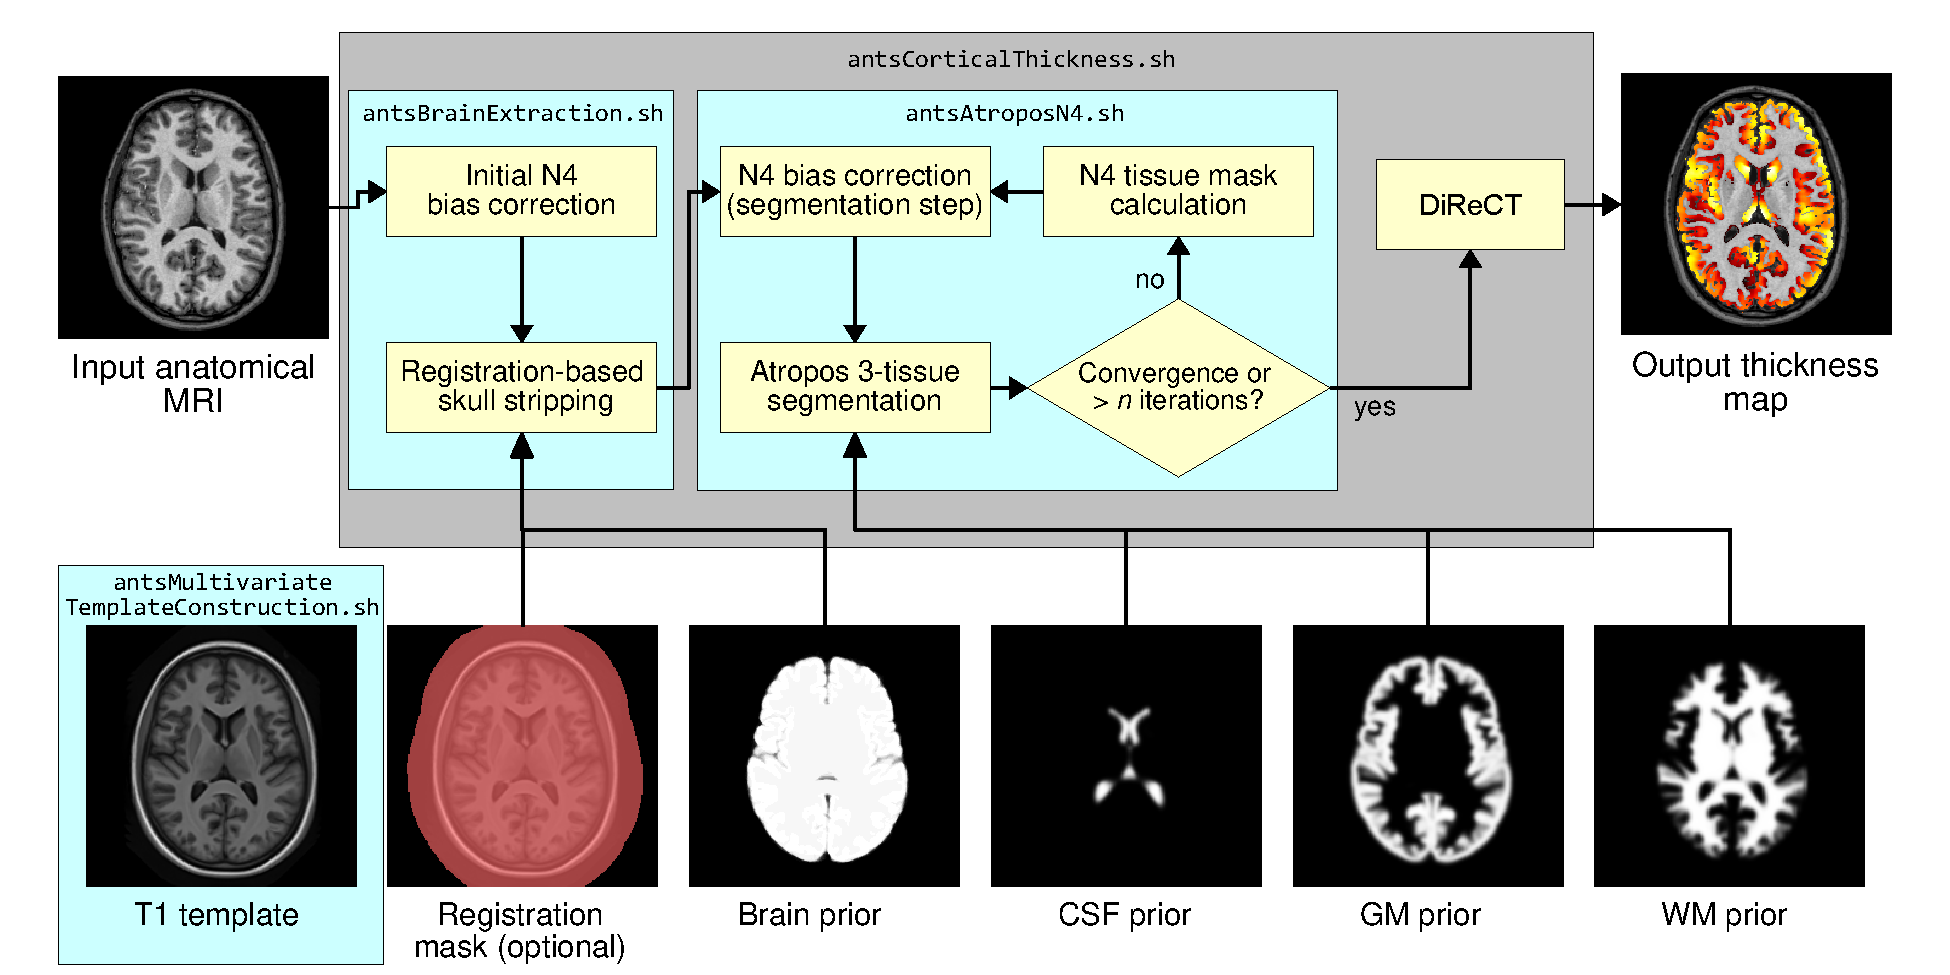
\includegraphics[width=180mm]{Figures/Kapowski_pipeline2.pdf}
  \caption{Illustration of the main components of the ANTs processing 
  workflow containing all elements for determining cortical thickness. 
  We also included the domain of operations for the selected scripts.
  Not shown is the optional subject to template registration.}
  \label{fig:pipeline}
\end{figure*}

\subsubsection{Anatomical template construction}

Normalizing images to a standard coordinate system
reduces intersubject variability in population studies.  Various
approaches exist for determining the normalized space such as the selection
of a pre-existing template based on a single subject, e.g. the Talairach
atlas \citep{Talairach1988}, or a publicly available averaged group of
subjects, e.g. the MNI \citep{Collins1994} or ICBM \citep{Mazziotta1995}
templates.  Additionally, mean templates constructed from labeled
data can be used to construct spatial priors for improving segmentation
algorithms.
The work of \cite{avants2010} explicitly models the geometric component of the 
normalized space during optimization to produce such mean templates.  Coupling the intrinsic symmetry of 
SyN pairwise registration \citep{avants2011} and an
optimized shape-based sharpening/averaging of the template appearance, Symmetric Group
Normalization (SyGN) is a powerful framework for producing optimal population-specific
templates.

%One challenge with standard templates is that they may inadvertently bias one's results by enabling better normalization of subjects to which the template is more similar.  This issue is exacerbated when dealing with populations that have high variance (e.g. due to disease) and/or when one's normalization method is low-dimensional (not flexible enough to capture large shape differences). 

%Population-specific templates alleviate some of
%the issues with other template approaches by deriving a most representative image from the population
%\citep{Good2001}.  Large deformation registration algorithms also reduce
%this confound by being less sensitive to the deformation distance
%between subject and target.  Some approaches combine both advantages,
%for instance, the diffeomorphic approach of Joshi et al. employs the
%SSD metric and a shape distance to bring the subject group of images
%into alignment \citep{Joshi2004}.  Variants
%include extension to multiple modalities \citep{Lorenzen2006} and small deformations
%\citep{Geng2009}.  These approaches iteratively minimize group difference in ``congealing''
%towards a representative image template \citep{Learned-Miller2006}.


The ANTs implementation of this technique is currently available as a shell script, 
\verb#buildtemplateparallel.sh#.  A generalized, multivariate version is also available as
\verb#antsMultivariateTemplateConstruction.sh#.  Both scripts are distributed as part of
 the ANTs repository.
The multivariate script permits the construction of multimodal templates (e.g. 
T1-weighted, T2-weighted, proton density MRI and fractional anisotropy).  
Both scripts accommodate a variety of computational resources
for facilitating template construction.  These computational resource possibilities include:
\begin{itemize}
  \item serial processing on a single workstation, 
  \item parallelized processing on a single workstation with multiple cores using \verb#pexec#%
  \footnote{http://www.gnu.org/software/pexec/pexec.1.html},
  \item parallelized processing using Apple's XGrid technology%
  \footnote{https://developer.apple.com/hardwaredrivers/hpc/xgrid\_intro.html}, 
  \item parallelized processing using Sun Grid Engine for cluster-based systems%
  \footnote{http://www.oracle.com/technetwork/oem/grid-engine-166852.html}, and 
  \item parallelized processing using the Portable Batch System for cluster-based systems%
  \footnote{http://www.pbsworks.com/}.
\end{itemize}

For this work, database-specific templates were used during cortical thickness pipeline
processing for both brain extraction and brain segmentation steps.  Multivariate templates 
were constructed from the multimodal data sets.  However, their usage was based on the 
fact that they had been built previously for other work and not because they provide a 
discernible advantage over univariate templates (i.e. T1-only) for the proposed workflow.

%Given a set of representative images, 
%$\{I_1, I_2, \ldots, I_M\}$, optimization involves finding the set of paired
%diffeomorphic transformations, $\left\{\left(\phi^1_1, \phi^1_2\right), 
%\left(\phi^2_1, \phi^2_2\right), \ldots, \left(\phi^M_1, \phi^M_2\right) \right\}$,
%the optimal template appearance, $J^*$, and corresponding coordinate system, $\psi(\mathbf{x})$,
%which minimize the following cost function:
%\begin{align}
%  \sum_{m=1}^M \left[
%    D\left( \psi(\mathbf{x}), \phi^m_1(\mathbf{x}, 1) \right) + 
%    \Pi \left( I_m\left(\phi^m_2(\mathbf{x}, 0.5) \right), J^*\left(\phi^m_1(\mathbf{x}, 0.5) \right) \right)
%    \right]
%\end{align}
%where $D$ is the diffeomorphic shape distance, 
%\begin{align}
%  D\left(\phi(\mathbf{x}, 0), \phi(\mathbf{x}, 1)\right) = \int_{0}^1 \| v(\mathbf{x}, t) \|_L dt, 
%\end{align}
%dependent upon the choice of the linear operator, $L$, and
%$v$ is the diffeomorphism-generating velocity field, 
%\begin{align}
%  v\left(\phi(\mathbf{x}, t), t \right) = \frac{d\phi(\mathbf{x}, t)}{dt},\,\,\, \phi(\mathbf{x}, 0) = \mathbf{x}.
%\end{align}
%$\Pi$ is th
%e choice of similarity metric, often cross-correlation \citep{Avants2008a}, calculated in the 
%virtual domain midway between each individual image and the current estimate of the template. 
%
%With initial assignment of $\left\{\left(\phi^m_1, \phi^m_2\right)\right\}$ and $\psi(\mathbf{x})$ 
%to identity, iterative optimization
%involves estimating the pairwise transformations, estimation of the optimal template appearance, and 
%updating $\psi(\mathbf{x})$ by averaging the current estimate of $\left\{\phi_1^m\right\}$.  


\subsubsection{N4 Bias field correction}

Critical to quantitative processing of MRI is the minimization of
field inhomogeneity effects which produce artificial low frequency 
intensity variation across the image.  Large-scale studies, such
as ADNI, employ
perhaps the most widely used bias correction algorithm, N3 \citep{sled1998}, 
as part of their standard protocol \citep{boyes2008}.

In \cite{tustison2010}, we introduced an improvement of N3, denoted as
``N4'', which demonstrates a significant increase in performance and convergence behavior
on a variety of data.  This improvement is a result of an enhanced 
fitting routine (which includes multi-resolution capabilities) and a modified optimization 
formulation.  For our workflow, the additional possibility of specifying
a weighted mask in N4 permits the use of a ``pure tissue'' probability map 
(described below)
calculated during the segmentation pipeline for further improvement of 
bias field estimation.  In addition to its public availability 
through ANTs and the Insight Toolkit, it has also been included in
the popular open source Slicer software package for visualization and medical
image computing \citep{fedorov2011}.

N4 is used in two places during the individual subject processing (cf Figure
\ref{fig:pipeline}).  
%
%% We don't need the following comment because none of the data were dicim
%% to begin with
%
%Following conversion of the raw dicom T1-weighted image
%to Nifti format using our related \verb#Neuropipedream# set of raw image conversion
%and organization tools%
%\footnote{
%http://sourceforge.net/projects/neuropipedream/
%}, 
Initially, it is used to generate an initial bias corrected image for use in
brain extraction.  The input mask is created by adaptively thresholding 
the background from the foreground using Otsu's algorithm \citep{otsu1979}.
Following brain extraction, four-tissue segmentation involves iterating
between bias field correction using the current pure tissue 
probability map as a weight mask and then using that bias corrected image
as input to the Atropos segmentation step (described below). 

\subsubsection{Brain extraction}

Brain extraction using ANTs combines template building, high-performance
brain image registration, and Atropos with topological refinements.  
An optimal template for brain extraction is 
generated offline using labeled brain data.  
In this work we use each cohort to produce a population-specific template 
(cf Figure \ref{fig:template}) and corresponding brain and four-tissue probability
maps (cf Figure \ref{fig:templateMasks}). 

  The warped brain probability map is thresholded at 0.5 and the resulting mask is dilated
with a radius of 2.  Atropos is used to generate an initial three-tissue segmentation estimate within the mask
region.  Each of the three tissue labels undergo specific morphological operations which are then
combined to create a brain extraction mask for use in the rest of the
cortical thickness workflow.  

A comparison of an earlier version of our extraction methodology 
using open access brain data with publicly available
brain extraction algorithms including AFNI's \verb#3dIntracranial#
\citep{ward1999}, FSL's \verb#BET2# \citep{smith2002}, Freesurfer's
\verb#mri_watershed# \citep{segonne2004}, and BrainSuite
\citep{dogdas2005} demonstrated that our combined
registration/segmentation approach \citep{avants2010a} performs at the
top level alongside BrainSuite (tuned) and FreeSurfer.



\subsubsection{Atropos four-tissue segmentation}

In \cite{avants2011a} we presented an open source $n$-tissue segmentation software tool
(which we denote as ``Atropos'') attempting to distill 20+ years of active research in this area
particularly some of its most seminal work (e.g. \cite{zhang2001,ashburner2005}). 
Specification of prior probabilities includes spatially varying Markov Random Field modeling, 
prior label maps, and prior probability maps typically derived from our template building 
process.  Additional
capabilities include handling of multivariate data, 
partial volume modeling \citep{shattuck2001}, a memory-minimization mode,
label propagation, a plug-n-play architecture for incorporation of novel likelihood models
which includes both parametric and non-parametric models for both scalar and tensorial
images, and alternative posterior formulations for different segmentation tasks.

Due to the important interplay between segmentation and bias correction,
we perform multiple N4 $\rightleftharpoons$ Atropos iterations.
In order to better integrate Atropos and N4, we use  
a pure tissue probability weight mask generated from the 
posterior probabilities derived from the segmentation 
step.  Given $N$ labels and the corresponding $N$
posterior probability maps $\{ P_1, \ldots, P_N\}$ produced
during segmentation, the N4 weight mask is 
created at each N4 $\rightleftharpoons$ Atropos iteration from
\begin{align}
  P_{pure\,\,tissue}(\mathbf{x}) = \sum_{i=1}^N P_i(\mathbf{x}) \prod_{j=1, j \neq i}^N \left( 1 - P_j(\mathbf{x}) \right).
\end{align}
One of the key insights of the original N3 development is the
observation that inhomogeneities cause the intensity values of
pure tissue peaks to spread in the intensity histogram as though
convolved with a Gaussian.  A core contribution of N3 is the
proposed corrective of deconvolving the intensity histogram to 
accentuate the tissue peaks coupled with a spatial smoothing 
constraint. The pure tissue probability mask
weights more heavily the voxels corresponding to pure tissue 
types (as determined by the segmentation) during the deconvolution process 
while minimizing the contribution of regions such as the gray/white matter 
interface where peak membership is ambiguous. 

Atropos enables prior knowledge to guide the
segmentation process where template-based priors are integrated into the optimization
with a user-controlled weight.  Modulating the likelihood and prior contributions
to the posterior probability is essential for producing adequate segmentations.
Atropos weights the likelihood and priors according to
\begin{align}
P(y|x) \propto P(y|x)^{1-\alpha}P(x)^{\alpha}
\end{align}
where $\alpha$ is a user-selected parameter which weights the tradeoff between the likelihood and priors terms.
In this work, we chose a weighting of $\alpha = 0.25$ 
based on our extensive experimentation with different parameter weights.


\subsubsection{DiReCT (aka KellySlater/KellyKapowski) Cortical Thickness Estimation}

DiReCT was introduced 
in \cite{das2009} and made available in ANTs as the program \verb#KellySlater#.
Since then several improvements have been made and incorporated into the program
\verb#KellyKapowski#.%
\footnote{
Traditional academic discourse encountered in the published literature
rarely contextualizes peculiarities such as algorithmic nomenclature.
We briefly mention that
this was the source of a rare disagreement between the first and last authors
based, as many disagreements are, on a simple misunderstanding and not an
affronting existential statement concerning a certain favorite sitcom
of the first author's youth. 
}
Among the most significant advancements is that the more recent
implementation is multi-threaded, written in rigorous ITK coding style, and 
has been made publicly available through  ANTs complete with a unique user 
interface design developed specifically for ANTs tools.  

\subsection{Public Data Resources}

As mentioned previously, the four public data sets which were processed
using the previously described pipeline are:
\begin{itemize}
  \item IXI,
  \item Kirby,
  \item NKI, and
  \item Oasis.
\end{itemize}
In addition, we used the NIREP data set to produce cortical labels for 
each of the processed T1 images.  All five data sets are described below.

%\subsubsection{LPBA40 Data for Skull Stripping}
%
%For the brain extraction step
%we used the data from the LPBA40 repository \citep{shattuck2008}.
%These data consist of 40 high-resolution 3D Spoiled Gradient Echo
%(SPGR) MRI acquisitions which were manually labeled delineating
%56 brain structures.  Additional post processing 
%included automated brain extraction using FSL's brain extraction tool 
%\citep{smith2002} which was followed by manual corrections.  These
%40 brain masks are also included with the database.  
%
%All 40 subjects were used to create a population-specific
%unbiased average template \cite{avants2010}.  The brain masks corresponding 
%to the 20 subjects were warped to the template space using the 
%transforms derived during the template building process.  A template 
%probability mask was created by averaging the warped brain masks.
%For brain extraction of any single individual this ANTS-based LPBA40 template 
%is coarsely registered to the single subject brain.  The template
%probability brain mask is warped to the individual subject and 
%is used as the initial brain mask estimate.  As mentioned previously,
%Atropos and binary morphological operations are used to refine the
%brain mask estimate.

\subsubsection{NIREP Data for Cortical Labelings}

The Nonrigid Image Registration Evaluation Project (NIREP%
\footnote{
http://www.nirep.org/
}) 
is an ongoing framework for evaluating image registration algorithms \citep{christensen2006}.
The initial data set introduced into the project consists of 
16 (8 male and 8 female) high resolution skull-stripped brain 
data with 32 cortical labels (cf Table \ref{table:nirep_labels}) manually drawn using a 
published protocol.

Cortical label propagation to each individual subject for all data sets
described below was performed using the PICSL multi-atlas joint label fusion
algorithm described in \cite{wang2013} which recently led the competition
at the MICCAI 2012 Grand Challenge on Multi-Atlas Labeling%
\footnote{
https://masi.vuse.vanderbilt.edu/workshop2012/index.php/Main\_Page
}
and is also 
distributed with the ANTs toolkit.  Cortical thickness values are averaged
within each label for each subject using only the non-zero voxels from the cortical thickness map.

%Given the gray matter labels, the white matter and CSF were identified 
%for each of the 16 subjects using Atropos.  Similar to the LPBA40
%data set, a NIREP template was created from all 16 subjects and each of the
%warped labels were used to create probabilistic estimates of the 
%labeled region boundaries. These probability maps were used as 
%spatial prior probabilities during the four-tissue segmentation component
%of the pipeline.  Using SyN, the NIREP template is registered to the
%extracted individual subject brain which is followed by a warping of the 
%NIREP priors to the space of the individual subject.  The initial warped 
%white matter probability map is used as the weighted confidence mask 
%in the follow-up bias correction step.

\begin{table}
\centering
\begin{tabular*}{0.45\textwidth}{@{\extracolsep{\fill}} l l}
\toprule
  1) L occipital lobe & 2) R occipital lobe \\
  3) L cingulate gyrus & 4) R cingulate gyrus \\
  5) L insula gyrus & 6) R insula gyrus \\
  7) L temporal lobe & 8) R temporal lobe \\
  9) L superior temporal gyr. & 10) R superior temporal gyr. \\
  11) L infero temporal region & 12) R infero temporal region \\
  13) L parahippocampal gyr. & 14) R parahippocampal gyr. \\
  15) L frontal pole & 16) R frontal pole \\
  17) L superior frontal gyrus & 18) R superior frontal gyrus \\
  19) L middle frontal gyrus & 20) R middle frontal gyrus \\
  21) L inferior gyrus & 22) R inferior gyrus \\
  23) L orbital frontal gyrus & 24) R orbital frontal gyrus \\
  25) L precentral gyrus & 26) R precentral gyrus \\
  27) L superior parietal lobule & 28) R superior parietal lobule \\
  29) L inferior parietal lobule & 30) R inferior parietal lobule \\
  31) L postcentral gyrus & 32)   R postcentral gyrus \\  
\bottomrule
\end{tabular*}
\caption{The 32 cortical NIREP labels.  FIXME---this table should be
  replaced with or augmented by graphs of thickness for all 32 regions
  across age.}
\label{table:nirep_labels}
\end{table}

\subsubsection{Data for Pipeline Evaluation}

\begin{figure}
  \centering
  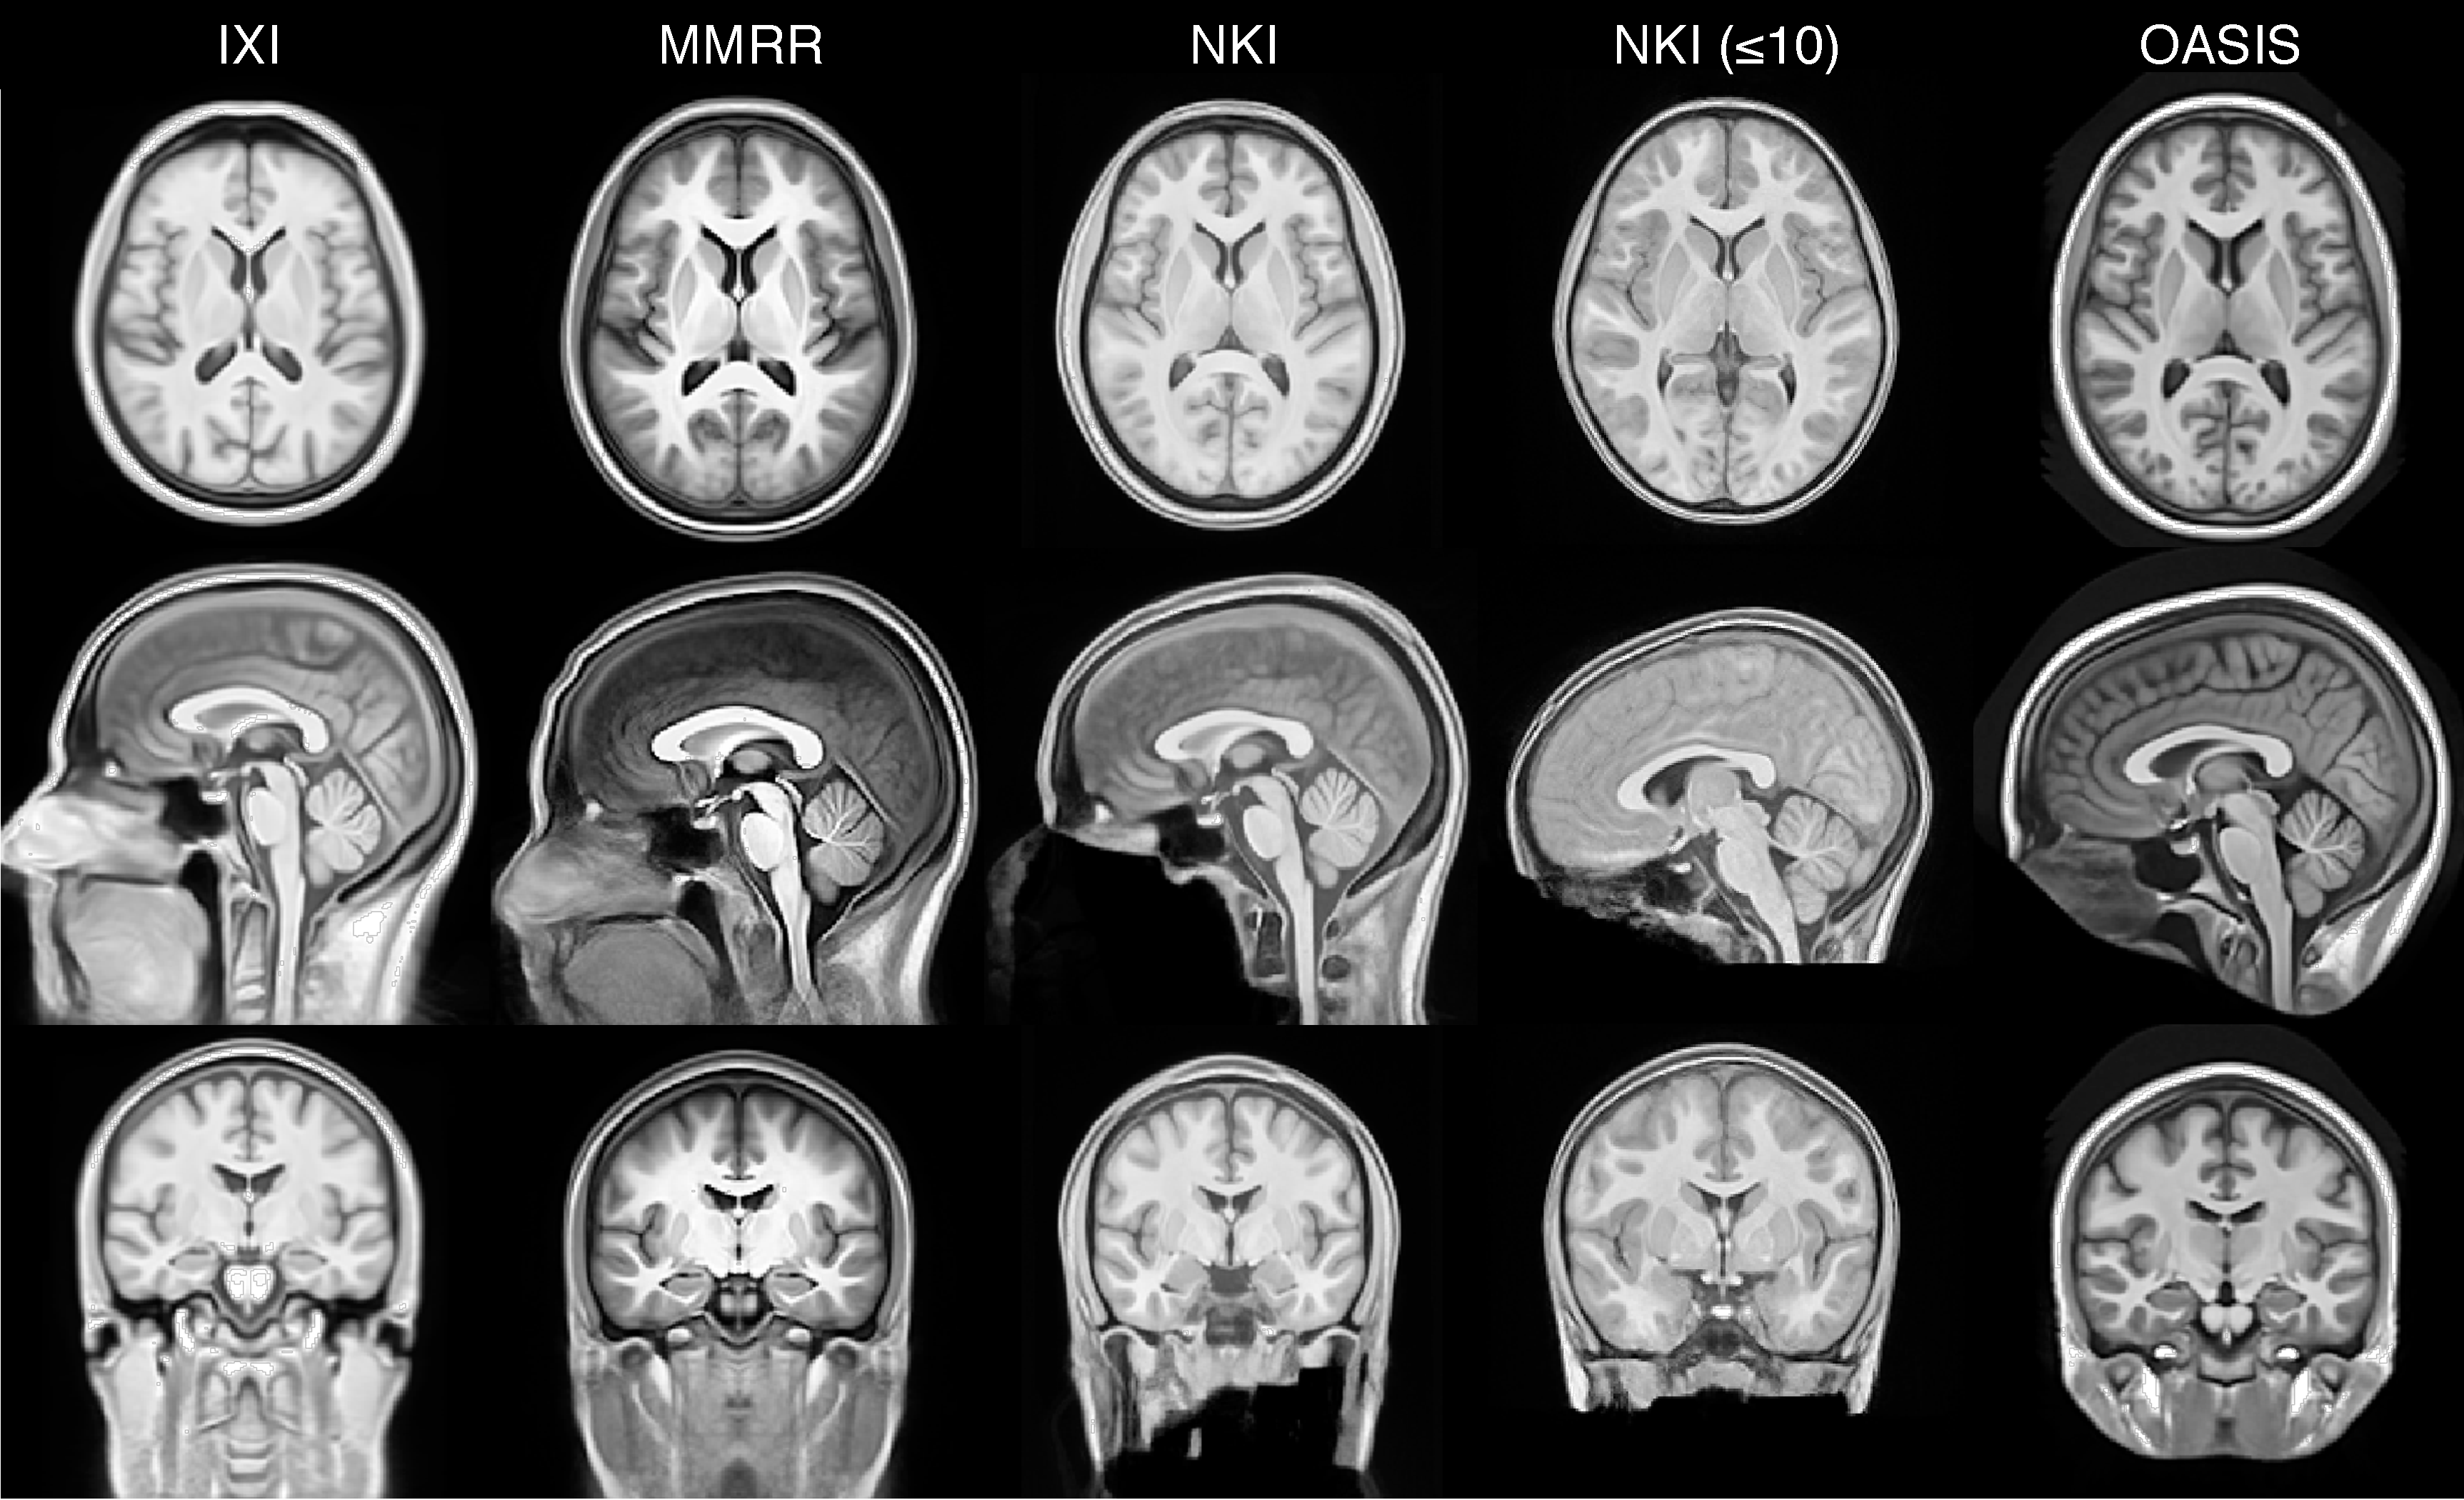
\includegraphics[width=90mm]{Figures/templates.pdf}
  \caption{Population-specific templates for each of the four public data sets used 
  for cortical thickness 
  estimation generated using the script antsMultivariateTemplateConstruction.sh. 
  The benefit of using such templates is obvious considering the variability in
  acquisition and data preparation (e.g. defacing protocols).
  }
  \label{fig:template}
\end{figure}

We apply the same pipeline to diverse publicly available datasets collected
from multiple sites and with a mixture of 3T and
1.5T T1 brain images.  Subjects in this dataset
span the age range from 4 to 96 years old.  This strategy tests robustness to
variation in head position, brain shape, defacing, image contrast, inhomogeneity, imaging
artifacts, and the broad variation in extracerebral tissue.  Failure
can occur in initial brain extraction, segmentation, registration, or
bias correction, any of which will lead to an inaccurate cortical
thickness measurement.                           

In total, we processed 1205 T1-weighted images from four different
public data sets to obtain the corresponding cortical thickness maps.                           
The descriptions of the four data sets are as follows: 
                                          
\paragraph{IXI}
Initially, we began with 581 T1-weighted images from the IXI%
\footnote{
http://biomedic.doc.ic.ac.uk/brain-development/
}
 data set
of which all were processed but only 563 subjects 
(313 females, 250 males) were included in the post processing analysis due to 
missing demographic information preventing an accurate estimate of 
the age at the time of image acquisition.  These data were
imaged at three sites 
with several modalities acquired (T1-weighted, T2-weighted, proton density, magnetic 
resonance angiography, and diffusion tensor imaging).  The 
database also consists of  demographic information such as date of birth, date
of scan, weight,
height, ethnicity, occupation category, educational level, and marital status.

\paragraph{Kirby}
The Multi-Modal MRI Reproducibility Resource%
\footnote{
http://www.nitrc.org/projects/multimodal/
}, 
or more informally, the Kirby
data set, was originally described in \cite{landman2011} consisting of 
21 subjects (10 females, 11 males) and features a rich multiple modality and 
repeated acquisition schedule.

\paragraph{NKI}
In support of open science, the 1,000 Functional Connectomes Project%
\footnote{ 
http://fcon\_1000.projects.nitrc.org
}
was initiated on December 11, 2009 by various members of the MRI community
seeking to form collaborative partnerships with imaging institutions for 
sharing well-documented multimodal image sets accompanied by phenotypic data.
One such contribution is the Nathan Klein Institute (NKI)/Rockland sample
consisting of 186 T1-weighted
images (87 females, 99 males).%
\footnote{
Downloaded on September 22, 2012.
}

\paragraph{Oasis}
The initial Open Access Series of Imaging Studies (OASIS)%
\footnote{
http://www.oasis-brains.org/
}
data set consisted of 433 T1-weighted images.  All were processed
although 100 subjects were excluded due to probable Alzheimer's
disease ($CDR > 0$) and 20 subjects had repeat scans
for 313 individual subjects included in the normal group statistical
analysis (118 males, 195 females).
Ages were between 18 and 96 and  
all subjects are right-handed.  
%Additional processing is included
%with the distribution including bias corrected and segmented images
%(gray, white and CSF matters).  


\begin{figure}
  \centering
  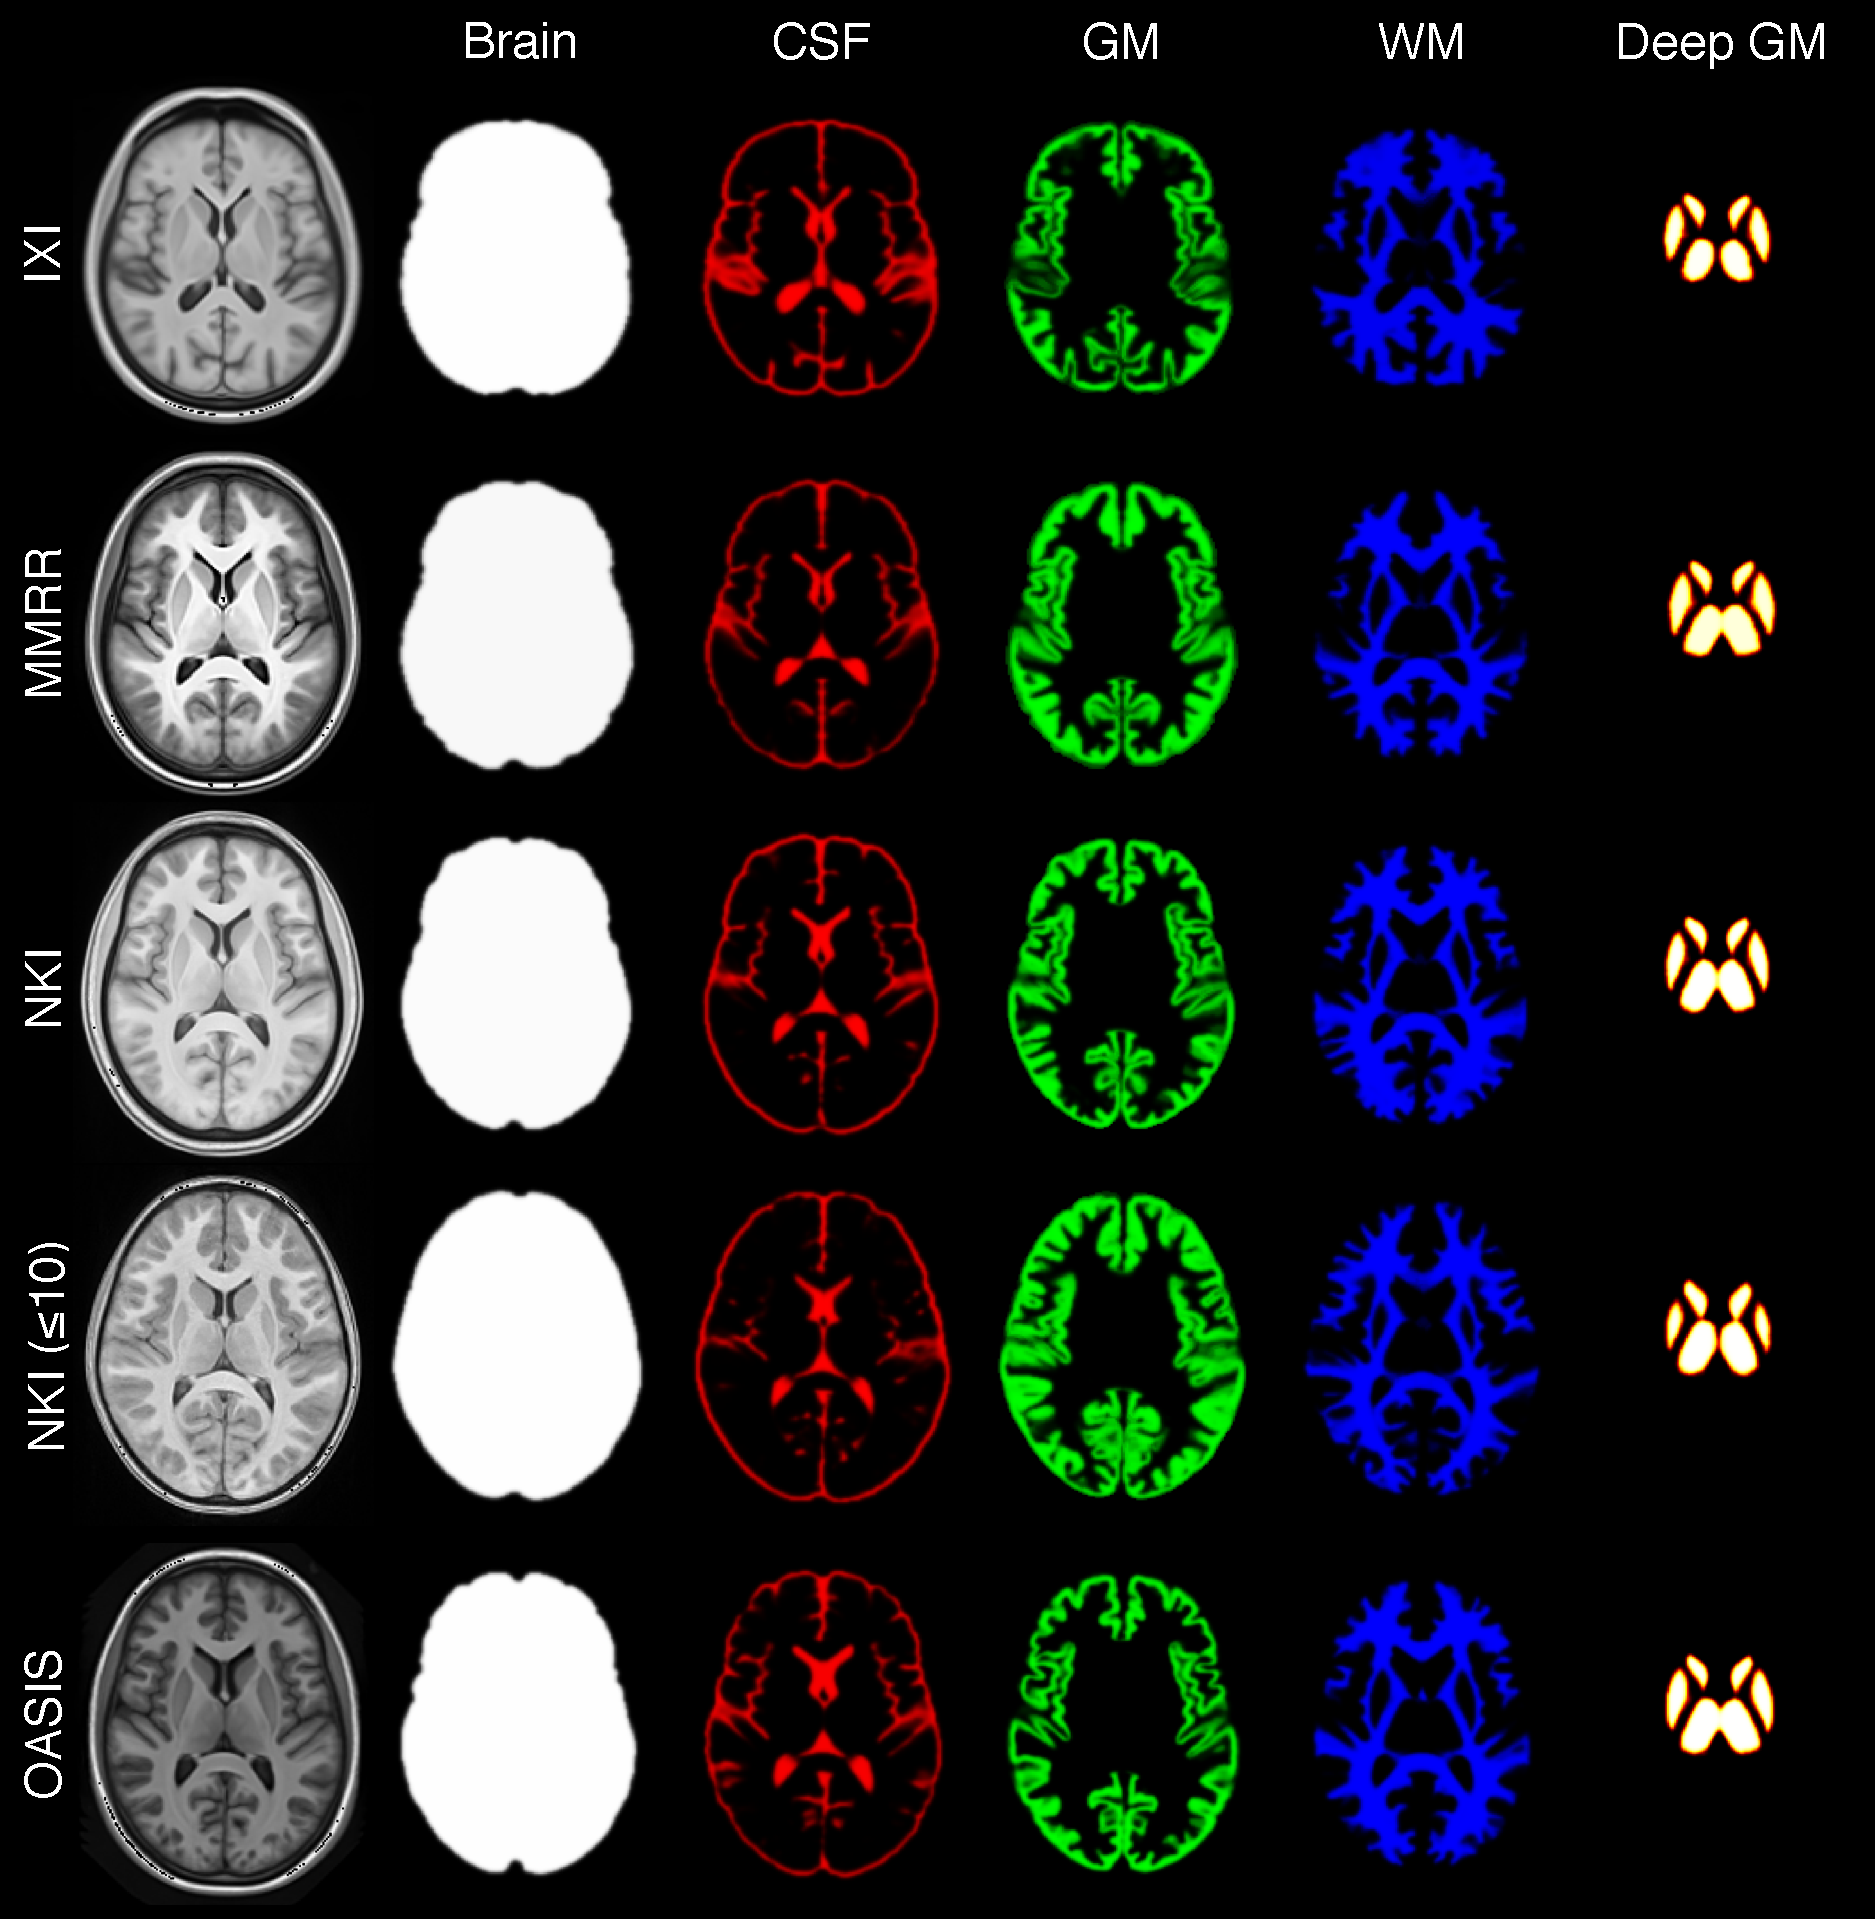
\includegraphics[width=90mm]{Figures/templateProbabilityMasks.pdf}
  \caption{Axial slices from each of the four T1 templates including the corresponding
  probability masks used for brain extraction and four-tissue brain segmentation.  
  }
  \label{fig:templateMasks}
\end{figure}




\section{Evaluation}
We cannot rely on traditional approaches such as manual
labeling to evaluate large-scale performance.  We therefore sought to
minimize failure rate, quantify the repeatability of cortical
thickness measures, test accuracy in BrainAGE \cite{franke2010} and
determine whether DiReCT reveals biologically plausible relationships
between the cortex, age and gender.  Collectively, these surrogate
measurements allow us to establish data-derived performance standards.

\subsection{Computation time \& Failure Rate}
All images underwent the pipeline processing illustrated in Figure 
\ref{fig:pipeline} using the computational cluster at the University 
of Virginia.%
\footnote{
http://www.uvacse.virginia.edu/itc-clusters/
}  
Processing times varied approximately between 10--20 hours per subject
for the entire cortical thickness estimation procedure.  The propagation of the
NIREP labels to each subject using label fusion as described earlier
was performed in parallel and took anywhere between 40 and 80 hours per 
subject.%
\footnote{
All processing was set to be single-threaded with a maximum requested memory 
footprint of 8 GB.
}  
Average thickness values were tabulated per subject for each of the
32 NIREP labels.  Cerebral volumes for each subject derived from the brain 
extraction step were also calculated.  All these data were written to separate csv
files corresponding to data set (also included with the scripts) for subsequent 
analysis.

We visually inspected the brain extraction, the estimated brain volume
and cortical thickness measurements for each of the 1205 images.  Out
of 1205 images, only 2 subjects failed (0.16\% failure rate).
\textcolor{red}{ Nick - can you explain this further ? Also - this
  might be a good place for registration, segmentation and thickness
  figures } Failures
occurred due to inaccurate brain extraction which is largely due to a
poor initial registration between the template whole head image and the
individual whole head image.  Failure did not occur
downstream from the brain extraction step.  

\subsection{Reproducibility}

\textcolor{red}{ Nick - do these vary with site , age or gender ?   it
  would be good to know how these variables affect reliability }

\begin{table}
\centering
\begin{tabular*}{0.9\textwidth}{@{\extracolsep{\fill}} l c c}
\toprule
\multicolumn{1}{c}{Region} & \multicolumn{1}{c}{Left} & \multicolumn{1}{c}{Right} \\
\midrule
occipital & $5.36 \pm 6.92$ & $5.79 \pm 7.17$\\
cingulate & $3.7 \pm 4.49$ & $3.62 \pm 4.6$\\
insula & $4.52 \pm 4.27$ & $4.43 \pm 4.36$\\
temporal pole & $4.93 \pm 5.48$ & $4.81 \pm 5.01$\\
superior temporal & $4.74 \pm 5.34$ & $3.58 \pm 4.92$\\
infero temporal & $6.86 \pm 8.8$ & $6.58 \pm 9.21$\\
parahippocampal & $5.13 \pm 5.29$ & $4.61 \pm 3.76$\\
frontal pole & $7.1 \pm 8.07$ & $7.4 \pm 8.32$\\
superior frontal & $3.86 \pm 4.48$ & $3.85 \pm 4.31$\\
middle frontal & $6.58 \pm 7.8$ & $5.87 \pm 7.96$\\
inferior & $4.53 \pm 5.53$ & $4.26 \pm 5.49$\\
orbital frontal & $4.77 \pm 6.12$ & $5.39 \pm 5.36$\\
precentral & $4.46 \pm 4.5$ & $4.15 \pm 4.81$\\
superior parietal & $3.71 \pm 4.14$ & $3.67 \pm 3.78$\\
inferior parietal & $4.96 \pm 6.06$ & $4.96 \pm 6.74$\\
postcentral & $5.51 \pm 6.32$ & $6.02 \pm 6.01$ \\
\bottomrule
\end{tabular*}
\caption{Mean percent variability error ($\pm$ standard deviation) of repeated 
cortical measurements for both the Oasis and Kirby repeat scans.
These differences were not statistically significant (two-tailed $t$-test
with false discovery rate (FDR) multiple comparisons correction).
}
\label{table:error}
\end{table}

Repeat scans of 40 subjects (20 Kirby subjects and 20 Oasis subjects) were 
used to determine the reproducibility of regional cortical thickness 
measurements. Similar to the assessment given in \cite{jovicich2013}, we
show regional reproducible thickness measurements, $T$, in terms of the
variability error:
\begin{align}
\varepsilon = \frac{|T_{scan} + T_{rescan}|}{0.5 \times (T_{scan} + T_{rescan})}
\end{align}
The error values for the 32 NIREP regions for both the Oasis and Kirby 
reproducibility data sets
are given in Table \ref{table:error}.  We also calculated the intraclass 
correlation coefficient 
(``ICC(2,1)'' in the notation of \cite{shrout1979}) to assess scan/rescan
reliability which showed reliable agreement ($ICC=0.95$).  

\subsection{BrainAGE Evaluation}


\begin{table}
\centering
\begin{tabular*}{0.9\textwidth}{@{\extracolsep{\fill}} l c c}
\toprule
\multicolumn{1}{c}{Analysis} & \multicolumn{1}{c}{$r$} & \multicolumn{1}{c}{mean error (years)} \\
\midrule
Gray matter probability & 0.93 & 6.17 \\  
Cortical thickness & 0.90 & 7.19 \\
\bottomrule
\end{tabular*}
\caption{Correlation and mean error values for both the gray matter probability and cortical thickness
{\it BrainAGE} evaluation.}
\label{table:brainAge}
\end{table}

\begin{figure*}
  \centering
  \begin{tabular}{cc}
  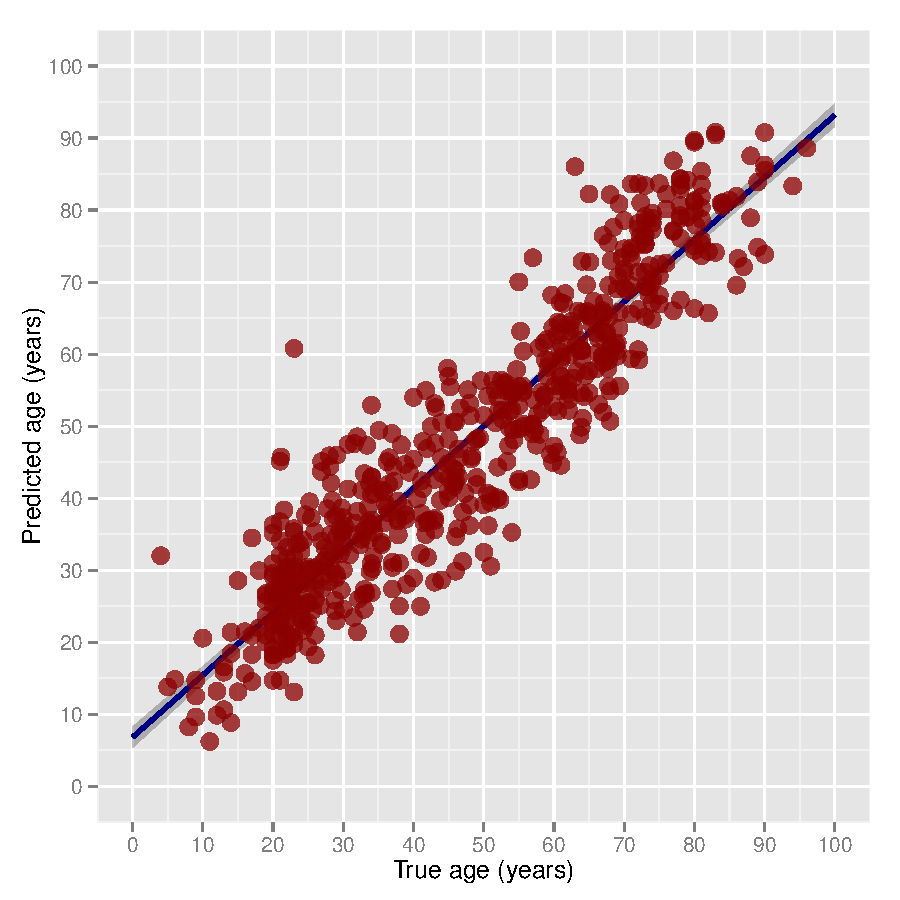
\includegraphics[width=65mm]{brainAgeBrainSegmentationPosteriors2.pdf} &
  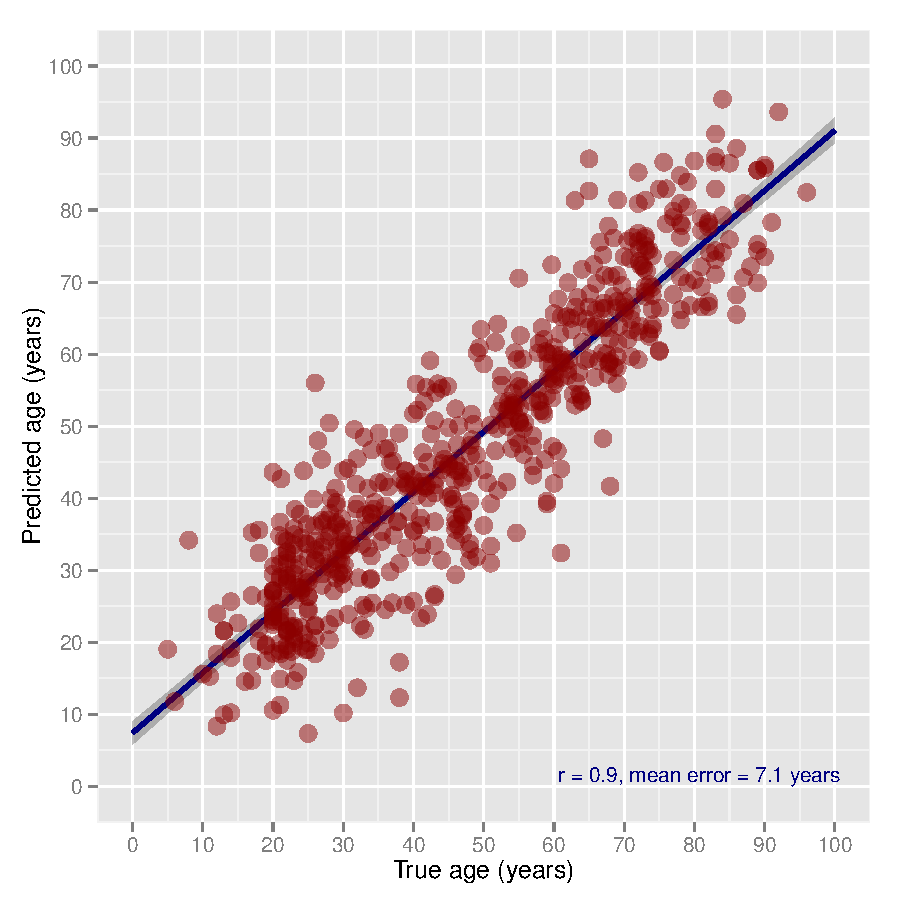
\includegraphics[width=65mm]{brainAgeCorticalThickness.pdf} \\
  (a) & (b) 
  \end{tabular}
  \caption{Results of RVM-based age prediction using (a) gray matter probability
  maps as in \cite{franke2010} and (b) cortical thickness maps both of which
  are derived from the previously described workflow.}
  \label{fig:brainAge}
\end{figure*}

In \cite{franke2010}, an estimation framework is presented for predicting 
apparent age from gray matter segmentation probability maps (denoted by the authors as {\it BrainAGE}).  
Given a normal age population spanning the age range of interest, the authors showed
how kernel regression methods can be used to reliably estimate age.  The basic processing pipeline includes 3-tissue segmentation
of a subject's T1, followed by registration to a common reference space (e.g.
the MNI template), smoothing (8 mm FWHM), and downsampling (8 mm 
isotropic resolution).  A principal components (PCA) model is constructed 
from the resulting aligned training image set.  The images of both the training set and 
testing set are decomposed into the bases of the PCA model which form the feature
set for relevance vector machine (RVM)-based learning and prediction, respectively. 

We applied the BrainAGE framework to the gray matter probability maps derived
from our pipeline.  We also applied the same strategy to predicting age from 
our cortical thickness images.  We randomly separated the images of each of the 
four cohorts into approximately two equal subgroups (testing and training).
Construction of the PCA model and decomposition of all images into the corresponding 
bases were performed on the training group using tools developed from the Insight Toolkit.%
\footnote{
http://www.itk.org/Doxygen/html/classitk\_1\_1ImagePCADecompositionCalculator.html  
}
We used the R-based {\it kernlab}%
\footnote{
http://rss.acs.unt.edu/Rdoc/library/kernlab/html/rvm.html
} 
package to train the RVM model and perform prediction.  Results for both
analyses  are shown in Fig. \ref{fig:brainAge} (cf. Fig. 3 in \cite{franke2010}).
Again, testing and training data, as well as 
R scripts used to produce the 
plots are publicly available.  
The resulting predictions for both image sets are quite similar as demonstrated 
visually in Fig. 3.  The correlation coefficients and mean errors in Table 
\ref{table:brainAge} between the
two approaches are also evidence of mutual corroboration.

\subsection{Gender and Age Relationships with DiReCT Cortical Thickness}

\textcolor{red}{ Nick - should just be basic regression results
  .... also allows us to look at site effect ... }
.....

\subsection{Gender Structural Connectivity Across Age Using Cortical Thickness}


\textcolor{red}{ Nick - should show a rendering of these networks -
  how about we residualize thickness wrt age and then look at the
  difference between male and female transitivity?  we can permute to
  get significance .... } 

\begin{figure*}
  \centering
  \begin{tabular}{c}
  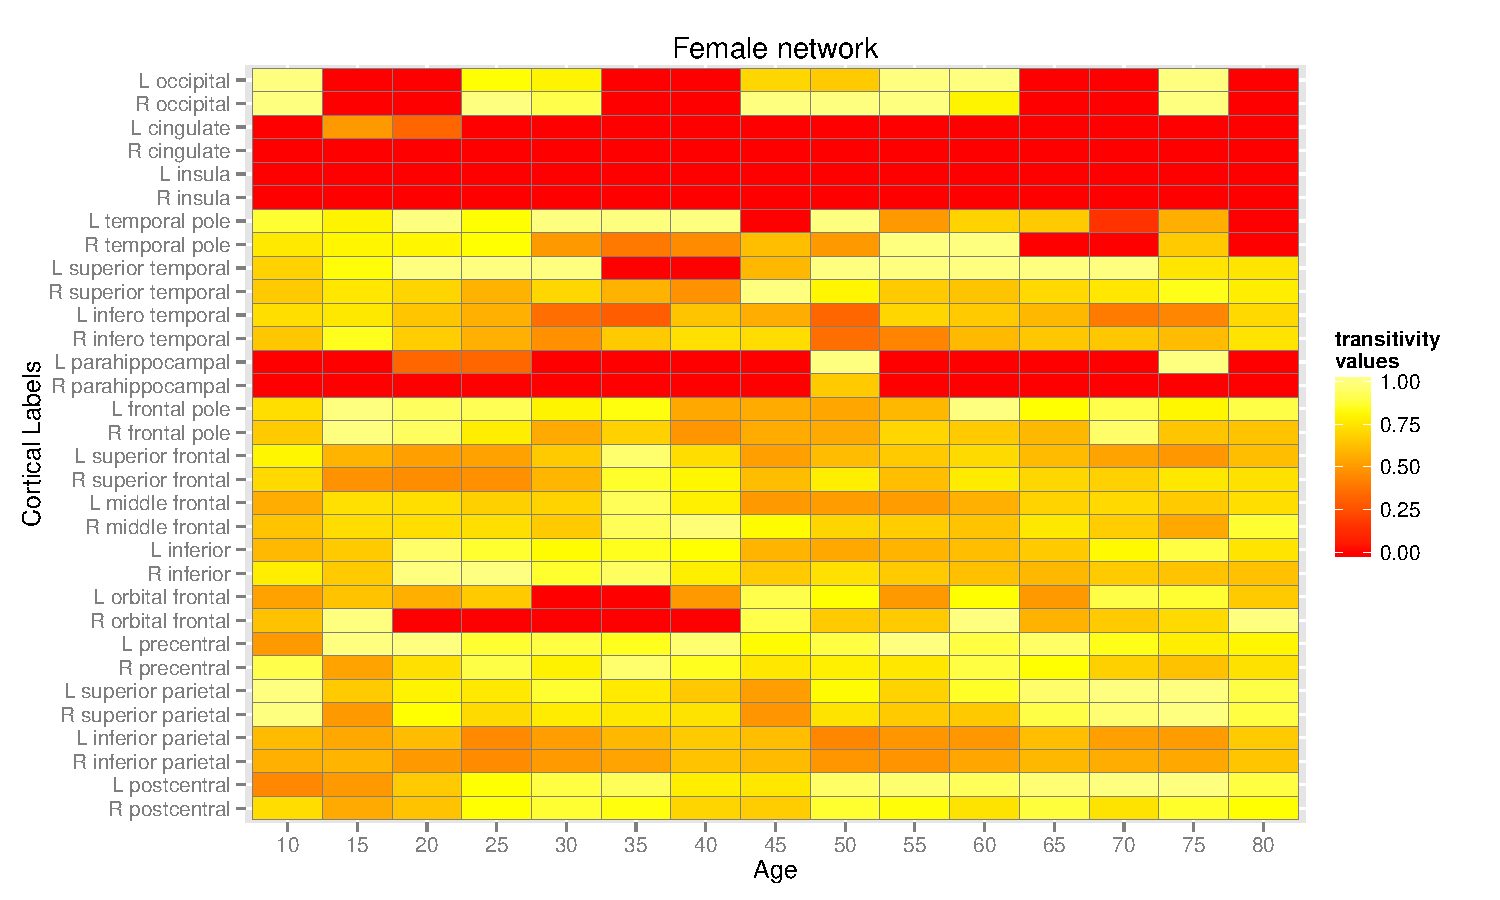
\includegraphics[width=140mm]{femaleNetwork.pdf} \\
  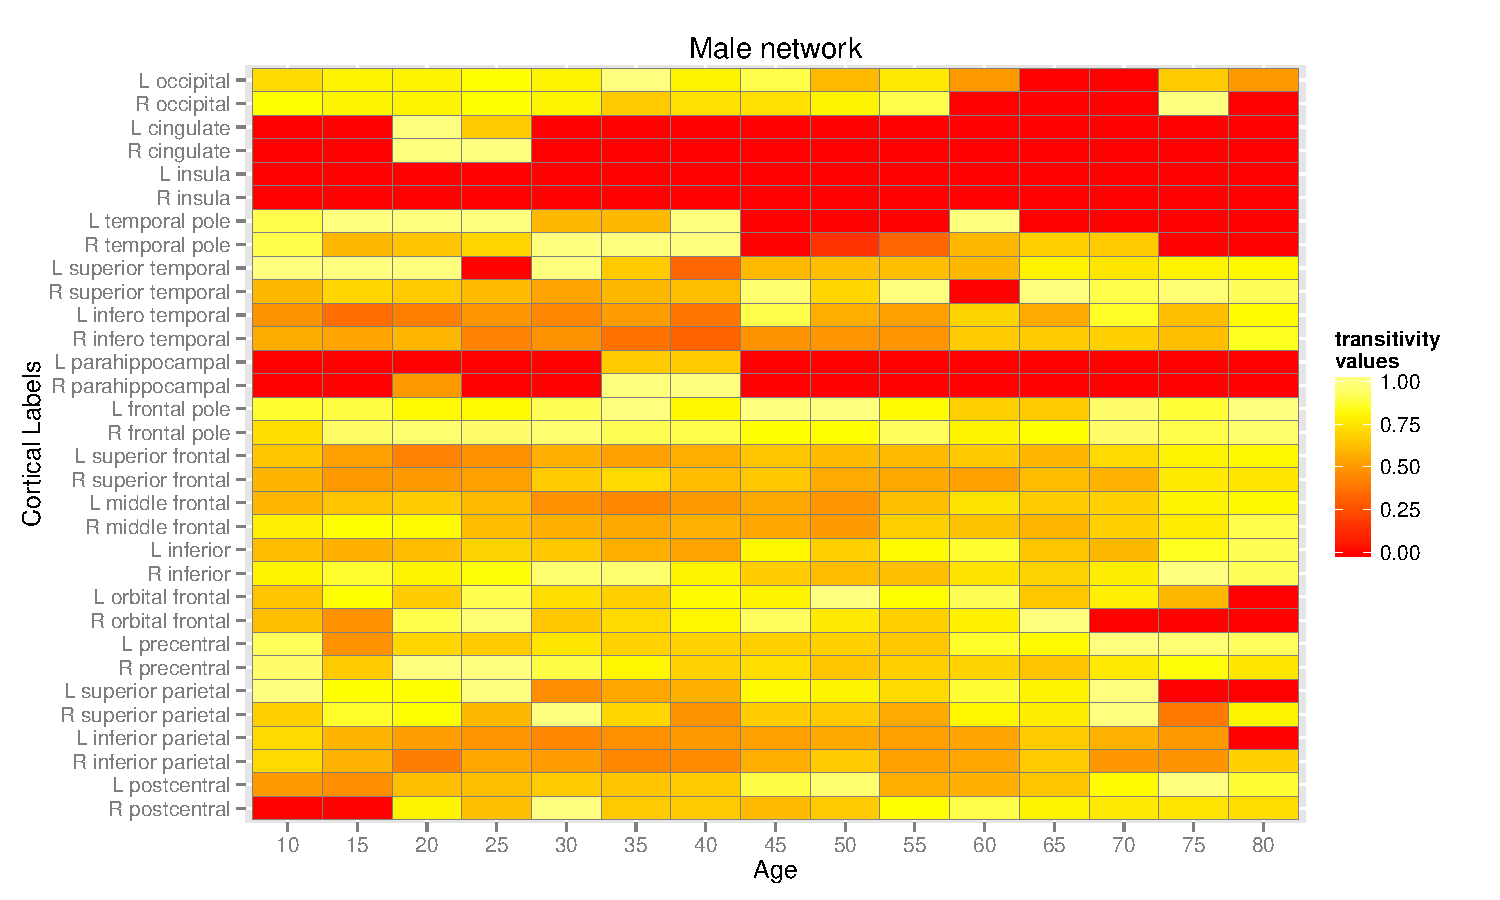
\includegraphics[width=140mm]{maleNetwork.pdf}
  \end{tabular}
  \caption{Transitivity (clustering coefficient) values across age for both the female (top)
  and male (bottom) networks.  
  }
  \label{fig:network}
\end{figure*}

As mentioned in the Introduction, cortical thickness has
been used to determine structural connectivity relationships in the brain 
where strong correlations in regional cortical 
thickness values across subjects provide evidence for anatomical
connectivity \citep{he2007,chen2008,he2008}.  Specifically, networks of neuronal
regions are thought to have small-world network properties \citep{sporns2004} 
in which clustered subnetworks are sparsely connected to other such clusters.
Measures such as the
clustering coefficient (or local transitivity) and mean shortest path length
\citep{watts1998}, are used to characterize networks in terms of their 
small-worldness.
%Although the principal purpose of this work is to showcase the 
%publicly available ANTs cortical thickness pipeline and its performance
%on open data
%(and not necessarily explore the deeper neuroscience implications of 
%the results), 
We use the compiled cortical thickness data to briefly sketch
the longitudinal variation in gender-based small-world networks of the
brain.  Note that these results are created directly from the tabulated 
cortical thickness values and processed with the R script
\verb#gender_study2.R#.

At each age between 10 and 80 years (in increments of 5), the weighted correlation
matrix for each gender is calculated from the thickness residuals 
(modeling the imaging acquisition site and total brain volume as covariates).  An undirected graph ($V \in$ \{NIREP regions\}, $E \in$ \{all NIREP pairings\})
is constructed from the correlation matrix where the graph density is specified at 25\%, i.e. only the nodal adjacencies corresponding to the top 25\% correlation values are used to create edges.    The local transitivity for a given vertex, $v_i$, with $k_i$ neighbors of the resulting graph is calculated from
\begin{align}
  transitivity(v_i) = \frac{|\{e_{jk}: v_j, v_k \in N_i, e_{jk} \in E \}|}{k_i (k_i-1)/2}.
\end{align}
Informally, this quantifies the proportion of edges between the neighbors of $v_i$ to the total number of possible edges in the neighborhood to quantify the proximity of the neighborhood to a complete graph.  Heat maps of the regional transitivity values for each
gender across age are given in Fig. \ref{fig:network}.  








\section{Discussion}

%Each test in the metrics
%
%We probably need a discussion section explaining why we chose each metric 
%
%Gender ... Brain extraction
%
%Brain age ... Bxt & affine reg and gm probs
%
%Constellations ... Segmentation & thickness 
%
%Repeatability ... thickness
%
%And what these metrics mean ... 
%
%I guess the networks "validate" thickness so maybe that's how we motivate them.



\section{Conclusions}

Imaging biomarkers such as cortical thickness play an 
important role in neuroscience research.  Extremely useful to
researchers are robust software tools for generating such 
biomarkers.  In this work we detailed our open source offering for estimating
cortical thickness directly from T1 images and demonstrated
its utility on a large collection of public brain data from
multiple databases acquired at multiple sites.  To our knowledge
this study constitutes the largest collection of cortical
thickness data processed in a single study.  
We expect that public availability of our tools and extensive tuning on 
the specified cohorts will prove useful to the larger
research community.  

In this work, we only explored a portion of the potentially
interesting investigations possible with these data.  However,
since all these data are publicly available, further work can
be easily pursued by us or even other interested groups.  We 
note that in addition to making the scripts, csv result files,
and cortical thickness maps available to researchers, 
posterior probability images are also offered permitting additional
quantification such as voxel-based morphometry \citep{ashburner2000}.


%% References with bibTeX database:

%\section*{Acknowledgments}

\section*{References}

\bibliographystyle{elsarticle-harv}
\bibliography{references}


%% Authors are advised to submit their bibtex database files. They are
%% requested to list a bibtex style file in the manuscript if they do
%% not want to use model1-num-names.bst.

%% References without bibTeX database:

% \begin{thebibliography}{00}

%% \bibitem must have the following form:
%%   \bibitem{key}...
%%

% \bibitem{}

% \end{thebibliography}


\end{document}

%%
%% End of file `elsarticle-template-1-num.tex'.
